\subsection{Deep Learning \index{Deep Learning}}
\label{sec:dl}

The Deep Learning module in TMVA provides the support to build several deep
learning architectures such as Deep Neural Networks (DNN), Convolutional networks (CNN) and
Recurrent networks (RNN).
The purpose of this module is to provide
optimized implementations of these networks
that can be efficiently trained on modern multi-core and GPU
hardware architectures.
For this,  the implementation provides two
backends for training and evaluating deep learning models.

The {\tt CPU} backend uses multithreading to perform
the training in parallel on multi-core CPU architectures and it can make use of  
efficient multithreaded BLAS implementations such as OpenBLAS and the Intel TBB library.

The {\tt GPU} backend can be used to perform the training on
CUDA-capable GPU architectures. In the case of Convolutional and Recurrent network models
the implementation uses the low level  CuDNN library of CUDA for optimal performances.


\paragraph{Building the CPU and GPU Backends}

%\hfill \break

To be able to use the multithreaded CPU backend, an implementation of the BLAS
library as well as the Intel TBB library must be available on the
system and detected by CMake. Note that the BLAS implementation must be
multithreaded in order to exploit the multithreading capabilities of
the underlying hardware.
The Intel TBB library  is used by the ROOT multi-threading libraries and it can be also part of
ROOT build. Note that the \code{IMT} CMake flag must be set
to enable multithreading in ROOT.
If a BLAS implementation is not available, but ROOT is built with support for
the MathMore library that is based on Gnu Scientific Library (GSL), the CBLAS implementation provided by GSL will be used .
If neither BLAS or CBLAS are found, then the native ROOT matrix package will be used for
the matrix multiplications needed to evaluate and train deep learning models.
If  ROOT has been built without IMT (multi-threading support) the execution will be serial instead of parallel. 

For the GPU backend, a CUDA installation is required on the system and
must be successfully detected by CMake. This requires the user to set the
\code{CUDA} CMake flag when installing Root.
Furthermore, for using CNN and RNN networks on GPU the CUDA cuDNN library
must be installed and detected by CMAKE (\code{CUDNN} CMAKE flag).  

If the user tries to use a backend that is not installed (e.g GPU), the training
of the DNN method will be performed using the alternative one (e.g. CPU). 



\subsubsection{Deep Neural Networks \index{Deep Neural Networks}}
\label {sec:dnn}

A \textit{deep neural network} (DNN) is an artificial neural network
(see Section~\ref{sec:ann}) with several hidden layers and a large
number of neurons in each layer. Recent developments in machine
learning have shown that these networks are capable of learning
complex, non-linear relations when trained on a sufficiently large
amount of training data. For an article describing the application of
DNNs to a classification problem in particle physics see the article
by Baldi, Sadowski and Whiteson \cite{higgs_dnn}.

The deep neural network implementation provides
an optimized implementation of feed-forward multilayer perceptrons
that can be efficiently trained on modern multi-core and GPU
architectures.

Note that previous ROOT/TMVA versions (version $<$ 6.22) provide for Deep Neural Networks a
method {\tt TMVA::kDNN}, implementing only fully connected layers.
Since ROOT version 6.18 it is recommended to use the new {\tt TMVA::kDL} method, which supports
not only dense layer as in the previous implementation, but also new type of layers as
convolutional and recurrent, allowing to build convolutional and recurrent networks, as
we will see in the next paragraphs.




\subsubsection{Training of Deep Learning Models}
\label{sec:dnn:update}

As common for deep neural networks, this implementation uses several
methods to train the network.
As example we report here the formula for the \textit{stochastic batch gradient descend} (SGD).
This means that in each training step the weights $W^k_{i,j}$ and bias
terms $\theta_{i}^k$ of a given layer $k$ are updated using

\begin{align}
  W^k_{i,j}   & \rightarrow W^k_{i,j}   - \alpha \frac{\partial J(\mathbf{x}_b, \mathbf{y}_b)}{\partial W^k_{i,j}} \\
  \theta^k_i & \rightarrow \theta^k_i - \alpha \frac{\partial J(\mathbf{x}_b, \mathbf{y}_b)}{\partial \theta^k_{i}}
\end{align}

Here $J(\mathbf{x}_b,\mathbf{y}_b)$ is the value of the loss function corresponding to
the randomly chosen input batch $\mathbf{x}_b$ and expected output
$\mathbf{y}_b$. If regularization is applied, the loss may as well contain
contributions from the weight terms $W^k_{i,j}$ of each layer. This implementation also supports training with momentum. In this case training updates take the form:

\begin{align}
  \Delta W^k_{i,j}   & \rightarrow p \Delta W^k_{i,j}   + (1.0 - p) \frac{\partial J(\mathbf{x}_b, \mathbf{y}_b)}{\partial W^k_{i,j}} \\
  W^k_{i,j}   & \rightarrow W^k_{i,j}   - \alpha \Delta W^k_{i,j} \\
  \Delta \theta^k_i & \rightarrow p \Delta \theta^k_i + (1.0 - p) \frac{\partial J(\mathbf{x}_b, \mathbf{y}_b)}{\partial \theta^k_{i}} \\
  \theta^k_i & \rightarrow \theta^k_i - \alpha \Delta \theta^k_i
\end{align}

Note that for $p = 0$ the standard stochastic batch gradient descent method is
obtained.

Other optimizer algorithms such as ADAM, which is the default one since ROOT version 6.18, ADAGRAD, RMSPROP and ADADELTA
are available as optmization algorithms, through the {\it Optimizer} option of the training strategy.
For a detailed description of the various method see ~\cite{dl_optimizers}.
%https://ruder.io/optimizing-gradient-descent/. 

The training batch $(\mathbf{x}_b,\mathbf{y}_b)$ is chosen randomly
and without replacement from the set of training samples. The number
of training steps necessary to traverse the whole training set one time is
referred to as an \textit{epoch}.

The training of the deep neural network is performed in one or
multiple training phases. A training phase ends when the test error
did not decrease for a user-specified number of epochs.

\paragraph{Validation and Evaluation Set}
\label{sec:dnn_test_and_evaluation_set}

The user should note that this implementation splits the TMVA training set in a sub-training set used to compute the gradient and update the weights and a validation set used to compute  the error and
to check for convergence. To properly evaluate the performance, the 
model is later  evaluated on a completely separate data set, the TMVA test set.

\subsubsection{Booking of the DL Method}

The booking of the DL method is similar to any other method in TMVA. The method
specific options are passed in the form of an option string \code{<options>} to
the method.

\begin{codeexample}
\begin{tmvacode}
factory->BookMethod(dataloader, TMVA::Types::kDL, "DNN", <options>);
\end{tmvacode}
\caption[.]{\codeexampleCaptionSize Booking of a deep neural network:
 The first argument is a \code{TMVA::DataLoader} object, which holds training and test
 data. The second argument is the predefined enumerator object that represents
 the deep neural network implementation. The third argument is a string holding
 a user defined name for the method. The fourth argument is the option string
 holding the options for the method. See Sec.~\ref{sec:usingtmva:booking}
 for more information on the booking.}
\label{example:DNN_booking}
\end{codeexample}

Through the option string, several configuration parameters can be specified.
The complete set of options that can be set in the options string are summarized in
Table~\ref{opt:mva:dnn:options}.
Some of the option such as the layout, define the models and the layers of the newtork and will be
described in greater details later, when describing the different deep leanring models that can be built.

The \code{Architecture} parameter is used to specify the backend used for the
training. The multi-core CPU and GPU backends must be enabled during the installation of Root
(CMAKE flgas {\code{tmva-cpu} and \code{tmva-gpu}). 

The method used to initialize the weight matrices before beginning the
training is specified using the \code{WeightInitialization}
argument. Possible values are \code{XAVIER}, which initializes the
weights with zero-mean Gaussian distributed random values, and
\code{XAVIERUNIFORM}, which initializes the weights with uniformly
distributed values.



\begin{option}[h]
\input optiontables/MVA__DNN_1.tex
\caption[.]{\optionCaptionSize
     Configuration options reference for MVA method: {\em DL}.
}
\label{opt:mva:dnn:options}
\end{option}

\subsubsection{Network Layout}
\label{sec:dnn:layout}

The structure of the deep learning model is specified by the
\code{Layout} parameter of the option string. This string specifies
the type of layer (e.g. dense, convolutional, recurrent ),
the activation function and some specific layer parameters such as the number of neurons of each layer of the
network or the filter sizes for the convolutional layers.  Different layers are separated by '\code{,}' characters while
layer parameter such as activation function and number of neurons are separated by '\code{|}'
characters.
Let's see in detail how to build the layout string for the different models..

\paragraph{Dense Layer Layout}

For example the layout string

\begin{tmvacode}
  Layout=TANH|128,TANH|128,TANH|128,LINEAR
\end{tmvacode}

defines a network with three hidden layers with 128 neurons and
$tanh$ activation functions. The neurons of the output layer are
inferred automatically from the number of classes (in the case of
classification) or the number of target variables (in the case of
regression).  
The available activation functions are given in
Table~\ref{opt:mva:dnn:activations}.

\begin{option}[h]
\input optiontables/MVA__DNN_2.tex
\caption[.]{\optionCaptionSize
     DL Activation Functions
}
\label{opt:mva:dnn:activations}
\end{option}


\subsubsection{Convolutional Networks \index{Convolutional Networks}}
\label {sec:cnn}

Convolutional Neural Networks are a popular variation of the feed-forward networks described in the previous section. By making the explicit assumption that the input is an image, they manage to
outperform conventional networks by significantly reducing the number of learnable parameters through a feature known as parameter sharing~\cite{alexnet}.
%%https://papers.nips.cc/paper/4824-imagenet-classification-with-deep-convolutional-neural-networks
Instead of connecting every neuron of the current layer with every neuron of the previous layer as in conventional dense layers,  we only learn the parameters for a set of a small kernels (typically
3x3 or 5x5) which slide over the input. The size of each kernel, as well as the number of pixels for each vertical or horizontal shift, are user defined meta-parameters. An important detail is that
while the model assumes spatial invariance with respect to the height and width, no such assumption is made with respect to the    mage depth. This asymmetry implies that at each receptive field, the kernel is connected with every slice of the input volume.

In order to reduce overfitting, we sometimes include a pooling layer between subsequent convolutional layers. This layer simply downsamples the input, typically by outputting the maximum value within
its receptive field. This does not only reduce the number of neurons, but also helps reduce overfitting. For more details the reader might find this paper~\cite{maxpool} informative. The meta-parameters of this
layer type are a subset of those of a convolutional layer, and are described in the section below.
%%%http://ais.uni-bonn.de/papers/icann2010_maxpool.pdf

\paragraph{Convolutional Network Layout}

A typical convolution network will first include several convolutional layers with different meta-parameters, each of them possibly followed by max-pooling layers to reduce overfitting. The last layers are fully connected (dense), in order to facilitate a soft-max activation similarly to traditional ANNs. An example layout configuration is depicted in the snippet below:


\begin{tmvacode}
Layout=CONV|12|3|3|1|1|1|1|RELU, CONV|12|3|3|1|1|1|1|RELU, MAXPOOL|2|2|2|2,
             RESHAPE|FLAT,DENSE|64|RELU,DENSE|1|LINEAR
\end{tmvacode}


Here we define a layout consisting of 2 convolutional layers, the last of which is followed by a pooling layer. After those layers, we include 2 fully connected layers where the last one consists of a
single neuron (binary classification). We also employ a flattening reshape layer necessary to connect the multi-dimensional output, produced by convolutional layers, to a dense layer.



Figure~\ref{fig''cnn_layer_layout}  visually explains the layout parameterization of the first convolutional layer.

\begin{figure}
\begin{center}
   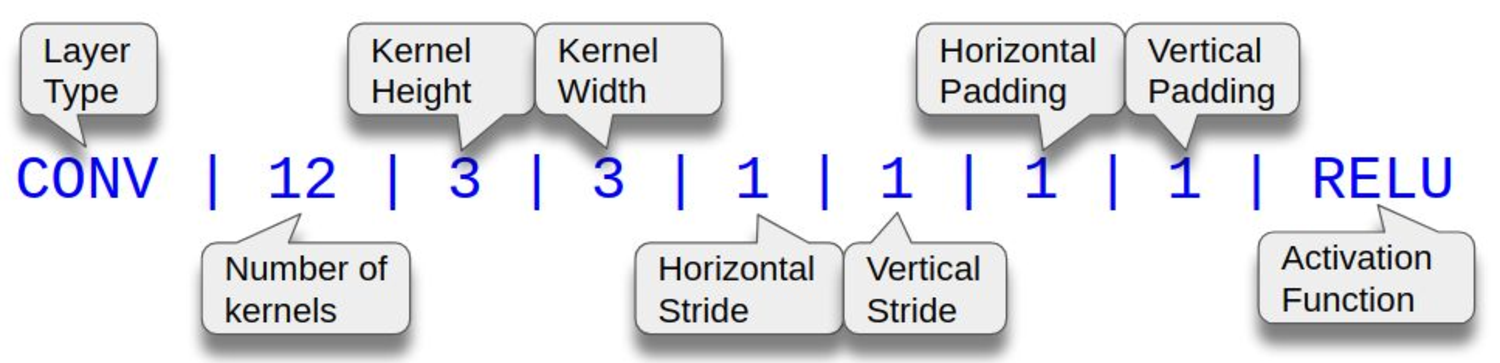
\includegraphics[width=0.9\textwidth]{plots/cnn-layer-layout.pdf}
   \label{fig:cnn_layer_layout}
   \caption{}
\end{center}
\end{figure}


\paragraph{Convolutional Layer Layout}

The parameters of the Convolutional layers are defined in the Layout string and they are separated by the '\code{|}' delimiter character.
Note that all of them must be provided. 
The parameters are the following, in order of occurence : 
\begin{itemize}
\item Layer Type (string) :   {\tt CONV}  for defining a  2D convolutional layer.
\item Number of kernels (integer),  {\it e.g.} 12 in the above example.
\item Filter height  (integer). 
\item Filter width (integer).
\item Vertical stride (integer).  Note that the stride must be a divisor of the input image size.
\item Horizontal stride (integer).  
 \item Vertical padding (integer)  The padding value has to be a valid one, i.e. it provides an output image size which is an  integer and not fractional.  See the formula below defining the output size
 \item  Horizontal padding (integer)
\item Activation function (string) : See Table~\ref{opt:mva:dnn:activations} for the list of possible activation functions.
\end{itemize}

  The Padding and stride parameter values must be consistent and have values that used with the given input image sizes and filter sizes result in integer output sizes and not fractional. 
  The formula that defines the output size is:
  
 \begin{equation}
    o = \frac{i - f + 2* p }{s} + 1
 \end{equation}
  where $o$ is the horizontal (or vertical) output size, $i$, $f$,$p$, $s$ are the corresponding input, filter, padding and stride sizes.
  In the example above with $f=3$, $s=1$,$p=1$ in both dimensions, the output image size will be equal to the input image size.

 \paragraph{MaxPool Layer Layout}

 The MaxPool layer is typically used in combination with convolutional layers in a CNN to down-sample the images.
 The MaxPool layer computes the maximum of the input in the provided rectangular pool size.
 The parameters describing the MaxPool layer are:
\begin{itemize}
\item Layer Type (string) :  {\tt MAXPOOL} for 2D max pooling layer.
\item Pool height dimension  (integer)  : {\it e.g.}  2 in the example above.
\item Pool width dimension  (integer).  
\item Vertical stride (integer).
\item Horizontal stride (integer).
\end{itemize}

Note that the output images after a maxpooling will be reduced(down-sampled) according to the following formula:

\begin{equation}
    o = \frac{i -f }{s} + 1
  \end{equation}
  
 \paragraph{Reshape Layer}

 The reshape layer is used to flatten the image that is the output from a convolutional layer or a maxpool layer in a format that can be input by a dense layer. After a convolution layer  the output
 data  will have a dimension equal to batch size $\times$ number of kernels $\times$ output height $\times$ output width ($B \times C \times H \times W$).  The reshape will reformat the data to a
 2-dimensional tensor (i.e. a matrix) with batch size as number of rows and 
 number of kernels $\times$ height $\times$ width as number of columns ( $B \times CHW$)  that can be processed by a dense layer.
 The reshale layer can also perform the inverse operation (de-flattening)

 The parameters of the reshape layers are different depending on the flattening or de-flattening case. In the flattening case the output depth, height and width can be omitted


 \begin{itemize}
\item Layer Type (string) :  {\tt RESHAPE}.
\item 1st output dimension (integer), e.g. output depth.
\item 2nd output dimension  (integer). 
\item 3rd output dimension (integer). 
\item string type: {\tt FLAT} for a flattening layer. In that case no need to specify the output dimension. 
\end{itemize}


\paragraph{Batch Normalization Layer}

The batch normalization layer normalizes the input by re-centering and re-scaling using the average and the standard deviation of the input batch. It is described in this paper~\cite{batch-norm}.
%%Ioffe, Sergey; Szegedy, Christian (2015). "Batch Normalization: Accelerating Deep Network Training by Reducing Internal Covariate Shift". arXiv:1502.03167
The parameters for this layer are:
\begin{itemize}
\item Layer type: {\tt BNORM}.
\item Momentum $\rho$, used for the running average (floating). Optional, default is $\rho = 0.99$.
\item $\epsilon$ parameter used for computing batchnorm (see formula in ~\cite{batch-norm}. Optional, default is $\epsilon=0.001$.
 \end{itemize}




\subsubsection{Recurrent Neural Networks \index{Recurrent Networks}}
\label {sec:rnn}

Recurrent neural network is a class of artificial neural networks where connections between nodes form a directed graph along a temporal sequence. This allows it to exhibit temporal dynamic
behavior. Different types of recurrent networks exist.
This implementation provides the support for 3 types of recurrent layers:
\begin{itemize}
\item Simple Recurrent layer (Vanilla RNN) as described for example in par. 10.2 of ~\cite{deeplearning_book}.
\item LSTM (Long Short-Term Memory) layer as defined in ~\cite{lstm}
\item GRU (Gate Recurrent unit) layer as defined in ~\cite{gru}
\end{itemize}

Here is an example of defining a recurrent neural networks composed of one LSTM layer followed by a dense layer for classification:

\begin{tmvacode}
  InputLayout=10|3:
  Layout=LSTM|12|3|10|0|1|RESHAPE|FLAT,DENSE|64|RELU,DENSE|1|LINEAR
\end{tmvacode}


The layer layout parameters for recurrent layers are

\begin{itemize}
 \item Layer Type (string) :  {\tt RNN} (Vanilla RNN), {\tt LSTM}, {\tt GRU}.
\item  Layer state size (integer).
\item  Input size  (integer)
\item  Time steps size  (integer), {\it i.e.} number of recurrent cells.
\item Remember state option (boolean), default is false (0). This corresponds to the stateful option in Keras.
\item Return the full output time sequence (boolean): default is false (0), i.e. return only output of last recurrent cell.
\item Reset  gate after option (boolean) : default is false. This is an option that applies only for GRU which defines a slightly different implementation..
  This option is forced to be true when using the GPU implementation, since it is the way cuDNN implements GRU. Note that with this option the GRU computation is slightly faster. 
\end{itemize}



\subsubsection{Input Layout}
\label{sec:dnn:inputlayout}


When using a convolutional or a recurrent network it is needed to provide an input layout string defining the format of the input, i..e. .its shape. In the case of convolutional networks  the size
of the input image (e.g. number of channels, image height, image width) must be defined and in the case of
recurrent networks we the time and the feature dimensions must be provided.
In the case of simple dense layer there is no need for an input layout because the total number of input event features can be deduced internally by TMVA..

The input layout shape is defined as following; here we give the example for input image with 3 channels, height = 32, width = 32: 

\begin{tmvacode}
InputLayout=3|32|32
\end{tmvacode}

The input layout parameters (input tensor dimensions) are separated as in the case of the layer layout by the '\code{|}' character.
For a RNN it is enough to provide an input layout of 2 dimensions: time and feature size.
For example for an RNN with an input dimension of 3 features in 10 time steps, we will have an input layout as following

\begin{tmvacode}
InputLayout=10|3
\end{tmvacode}  



\subsubsection{Training Strategy}
\label{sec:dnn:training}

The training of deep neural networks is performed in one or several
consecutive training phases that are specified using the
\code{TrainingStategy} argument of the \code{<options>} string passed
to the \code{BookMethod} call. A single phase is specified by the
parameters described in Table~\ref{opt:mva:dnn:training}. Different
training phases are separated by \code{|} characters.
 As an example, a valid training strategy string would be the following:

\begin{tmvacode}
  TrainingStrategy = LearningRate=1e-1,MaxEpoch=20
                   | LearningRate=1e-2, MaxEpoch=30
                   | LearningRate=1e-3, MaxEpoch=40
\end{tmvacode}

This training strategy trains the network in three training phases
each with a lower learning rate. This is particular useful if using the
$SGD$ optimizers which requires a manual adaptation of the learning rate.
When using instead an optimizer, such as $ADAM$, the  learning rate adapts automatically and there
is no such need to define several training strategies. 

Dropout is a regularization technique that with a certain probability
sets neuron activations to zero. This probability can be set for all
layers at once by giving a single floating point value or a value for
each hidden layer of the network separated by '\code{+}'
signs. Probabilities should be given by a value in the interval
$[0,1]$.

\begin{option}[h]
\input optiontables/MVA__DNN_3.tex
\caption[.]{\optionCaptionSize
     Configuration options reference for MVA method: {\em DL}.
}
\label{opt:mva:dnn:training}
\end{option}

\clearpage
